

\tikzset{every picture/.style={line width=0.3pt}} %set default line width to 0.75pt        

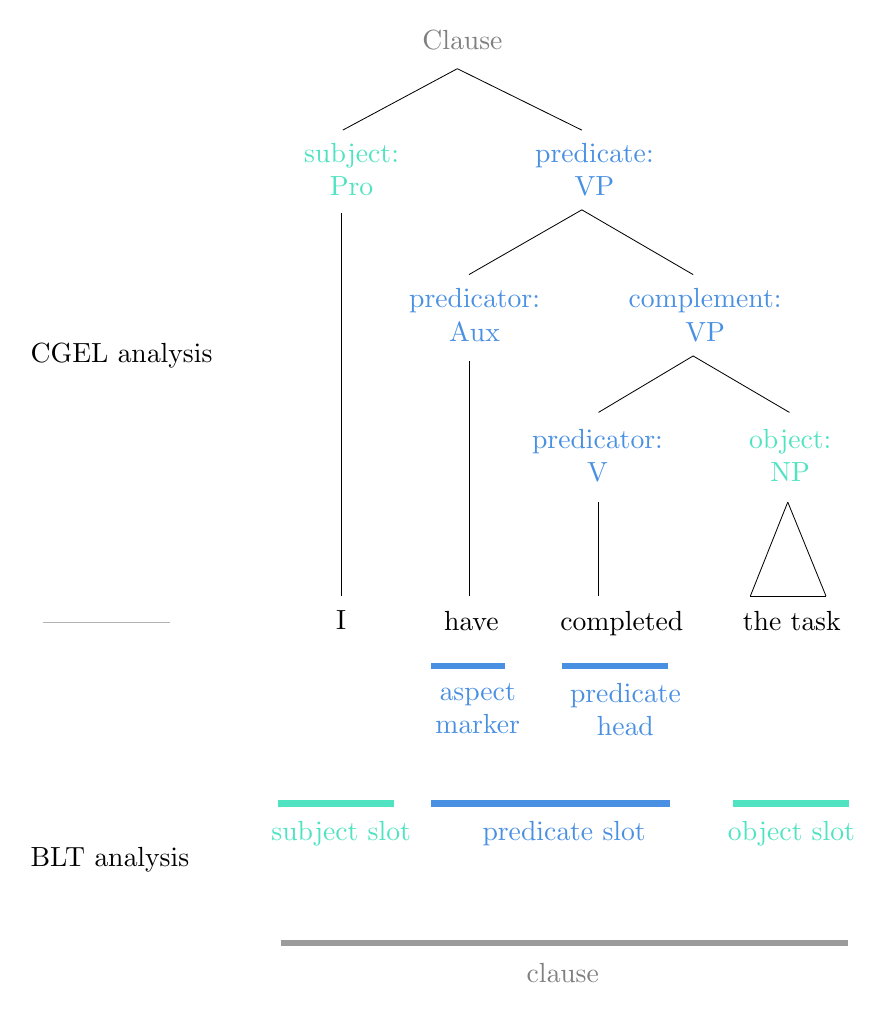
\begin{tikzpicture}[x=0.75pt,y=0.75pt,yscale=-0.8,xscale=0.8]
%uncomment if require: \path (0,700); %set diagram left start at 0, and has height of 700

%Straight Lines [id:da6978159989338242] 
\draw    (460.51,337.45) -- (438,394) ;
%Straight Lines [id:da25612792188160904] 
\draw    (483.51,394) -- (438,394) ;
%Straight Lines [id:da7073468356747876] 
\draw    (460.51,337.45) -- (483.51,394) ;
%Straight Lines [id:da49187631705005086] 
\draw    (346.51,394) -- (346.51,337.45) ;
%Straight Lines [id:da6438993209295902] 
\draw    (403.51,249.45) -- (346.51,283.45) ;
%Straight Lines [id:da38089606971298307] 
\draw    (403.51,249.45) -- (461.51,283.45) ;
%Straight Lines [id:da7906123481437248] 
\draw    (268.51,394) -- (268.51,252.45) ;
%Straight Lines [id:da8643521491921196] 
\draw    (336.51,161.45) -- (268.51,200.45) ;
%Straight Lines [id:da0004714779000363212] 
\draw    (336.51,161.45) -- (403.51,200.45) ;
%Straight Lines [id:da5878863240157226] 
\draw    (191.51,394) -- (191.51,163.45) ;
%Straight Lines [id:da007642253330256921] 
\draw    (261.51,76.45) -- (192.51,113.45) ;
%Straight Lines [id:da26086375276292184] 
\draw    (261.51,76.45) -- (336.51,113.45) ;
%Straight Lines [id:da012808187365270784] 
\draw [color={rgb, 255:red, 74; green, 144; blue, 226 }  ,draw opacity=1 ][line width=2.25]    (245.51,436) -- (290.51,436) ;
%Straight Lines [id:da08907193420089254] 
\draw [color={rgb, 255:red, 74; green, 144; blue, 226 }  ,draw opacity=1 ][line width=2.25]    (324.51,436) -- (388.51,436) ;
%Straight Lines [id:da4529555746551439] 
\draw [color={rgb, 255:red, 74; green, 144; blue, 226 }  ,draw opacity=1 ][line width=2.25]    (245.51,519) -- (389.51,519) ;
%Straight Lines [id:da6854837392493609] 
\draw [color={rgb, 255:red, 80; green, 227; blue, 194 }  ,draw opacity=1 ][line width=2.25]    (427.51,519) -- (497.51,519) ;
%Straight Lines [id:da2180304820675405] 
\draw [color={rgb, 255:red, 80; green, 227; blue, 194 }  ,draw opacity=1 ][line width=2.25]    (153.51,519) -- (223.51,519) ;
%Straight Lines [id:da8479817271509194] 
\draw [color={rgb, 255:red, 155; green, 155; blue, 155 }  ,draw opacity=1 ][line width=2.25]    (155.51,603) -- (496.51,603) ;
%Straight Lines [id:da08838256586100046] 
\draw [color={rgb, 255:red, 0; green, 0; blue, 0 }  ,draw opacity=0.3 ]   (12,410.09) -- (88.51,410.09) ;

% Text Node
\draw (187,401.5) node [anchor=north west][inner sep=0.75pt]   [align=left] {I};
% Text Node
\draw (252,401.5) node [anchor=north west][inner sep=0.75pt]   [align=left] {have};
% Text Node
\draw (322,401.5) node [anchor=north west][inner sep=0.75pt]   [align=left] {completed};
% Text Node
\draw (432,401.5) node [anchor=north west][inner sep=0.75pt]   [align=left] {the task};
% Text Node
\draw (433,292) node [anchor=north west][inner sep=0.75pt]  [color={rgb, 255:red, 80; green, 227; blue, 194 }  ,opacity=1 ] [align=left] {\begin{minipage}[lt]{33pt}\setlength\topsep{0pt}
\begin{center}
object:\\NP
\end{center}

\end{minipage}};
% Text Node
\draw (302,292) node [anchor=north west][inner sep=0.75pt]  [color={rgb, 255:red, 74; green, 144; blue, 226 }  ,opacity=1 ] [align=left] {\begin{minipage}[lt]{50.88pt}\setlength\topsep{0pt}
\begin{center}
predicator:\\V
\end{center}

\end{minipage}};
% Text Node
\draw (360,207.5) node [anchor=north west][inner sep=0.75pt]  [color={rgb, 255:red, 74; green, 144; blue, 226 }  ,opacity=1 ] [align=left] {\begin{minipage}[lt]{59.04pt}\setlength\topsep{0pt}
\begin{center}
complement:\\VP
\end{center}

\end{minipage}};
% Text Node
\draw (228,207.5) node [anchor=north west][inner sep=0.75pt]  [color={rgb, 255:red, 74; green, 144; blue, 226 }  ,opacity=1 ] [align=left] {\begin{minipage}[lt]{50.88pt}\setlength\topsep{0pt}
\begin{center}
predicator:\\Aux
\end{center}

\end{minipage}};
% Text Node
\draw (304,120) node [anchor=north west][inner sep=0.75pt]  [color={rgb, 255:red, 74; green, 144; blue, 226 }  ,opacity=1 ] [align=left] {\begin{minipage}[lt]{46.32pt}\setlength\topsep{0pt}
\begin{center}
predicate:\\VP
\end{center}

\end{minipage}};
% Text Node
\draw (165,120) node [anchor=north west][inner sep=0.75pt]  [color={rgb, 255:red, 80; green, 227; blue, 194 }  ,opacity=1 ] [align=left] {\begin{minipage}[lt]{37.58pt}\setlength\topsep{0pt}
\begin{center}
subject:\\Pro
\end{center}

\end{minipage}};
% Text Node
\draw (239,52) node [anchor=north west][inner sep=0.75pt]  [color={rgb, 255:red, 128; green, 128; blue, 128 }  ,opacity=1 ] [align=left] {Clause};
% Text Node
\draw (244,445) node [anchor=north west][inner sep=0.75pt]  [color={rgb, 255:red, 74; green, 144; blue, 226 }  ,opacity=1 ] [align=left] {\begin{minipage}[lt]{33.9pt}\setlength\topsep{0pt}
\begin{center}
aspect\\marker
\end{center}

\end{minipage}};
% Text Node
\draw (325,445) node [anchor=north west][inner sep=0.75pt]  [color={rgb, 255:red, 74; green, 144; blue, 226 }  ,opacity=1 ] [align=left] {\begin{minipage}[lt]{43.49pt}\setlength\topsep{0pt}
\begin{center}
predicate\\head
\end{center}

\end{minipage}};
% Text Node
\draw (272,528.5) node [anchor=north west][inner sep=0.75pt]  [color={rgb, 255:red, 74; green, 144; blue, 226 }  ,opacity=1 ] [align=left] {\begin{minipage}[lt]{62.79pt}\setlength\topsep{0pt}
\begin{center}
predicate slot
\end{center}

\end{minipage}};
% Text Node
\draw (420,528.5) node [anchor=north west][inner sep=0.75pt]  [color={rgb, 255:red, 80; green, 227; blue, 194 }  ,opacity=1 ] [align=left] {\begin{minipage}[lt]{49.47pt}\setlength\topsep{0pt}
\begin{center}
object slot
\end{center}

\end{minipage}};
% Text Node
\draw (145,528.5) node [anchor=north west][inner sep=0.75pt]  [color={rgb, 255:red, 80; green, 227; blue, 194 }  ,opacity=1 ] [align=left] {\begin{minipage}[lt]{54.05pt}\setlength\topsep{0pt}
\begin{center}
subject slot
\end{center}

\end{minipage}};
% Text Node
\draw (299,613.5) node [anchor=north west][inner sep=0.75pt]  [color={rgb, 255:red, 128; green, 128; blue, 128 }  ,opacity=1 ] [align=left] {\begin{minipage}[lt]{29.38pt}\setlength\topsep{0pt}
\begin{center}
clause
\end{center}

\end{minipage}};
% Text Node
\draw (3,240.09) node [anchor=north west][inner sep=0.75pt]   [align=left] {CGEL analysis};
% Text Node
\draw (3,544.09) node [anchor=north west][inner sep=0.75pt]   [align=left] {BLT analysis};


\end{tikzpicture}
